% Knowledge Graph Figure - can be included with \input{filename.tex}
\begin{figure}[htbp]
\centering
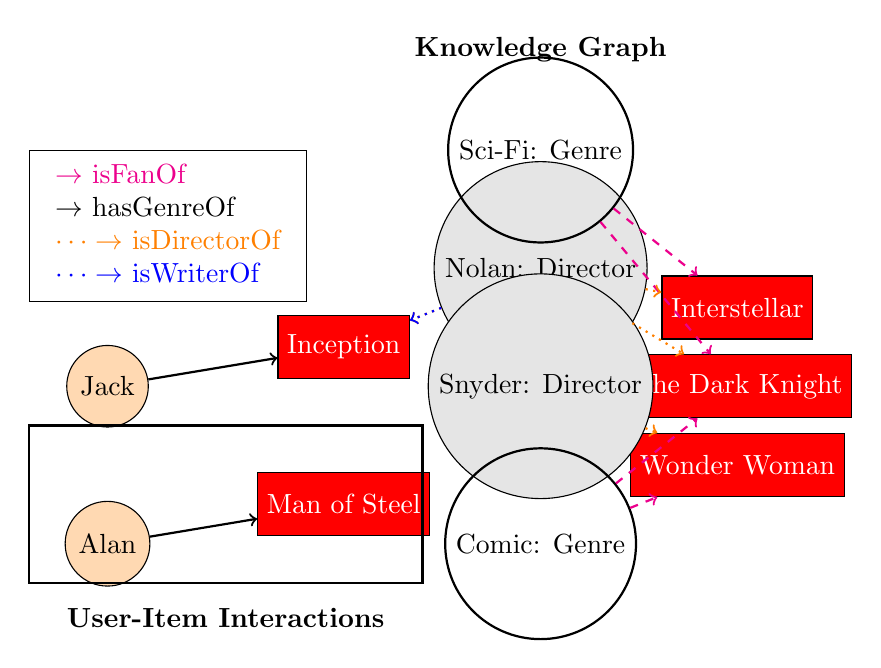
\begin{tikzpicture}[
    node distance=2cm,
    user/.style={circle, draw, fill=orange!30, minimum size=1cm},
    movie/.style={rectangle, draw, fill=red, text=white, minimum width=1.5cm, minimum height=0.8cm},
    person/.style={circle, draw, fill=gray!20, minimum size=1.2cm},
    genre/.style={circle, draw, thick, minimum size=1.2cm},
    arrow/.style={->, thick},
    dashed_arrow/.style={->, thick, dashed, magenta},
    dotted_arrow/.style={->, thick, dotted, orange},
    blue_dotted/.style={->, thick, dotted, blue}
]

% Users
\node[user] (jack) at (0,0) {Jack};
\node[user] (alan) at (0,-2) {Alan};

% Movies (YouTube icons represented as red rectangles)
\node[movie] (inception) at (3,0.5) {Inception};
\node[movie] (steel) at (3,-1.5) {Man of Steel};
\node[movie] (interstellar) at (8,1) {Interstellar};
\node[movie] (dark_knight) at (8,0) {The Dark Knight};
\node[movie] (wonder_woman) at (8,-1) {Wonder Woman};

% People
\node[person] (nolan) at (5.5,1.5) {Nolan: Director};
\node[person] (snyder) at (5.5,0) {Snyder: Director};

% Genres
\node[genre] (scifi) at (5.5,3) {Sci-Fi: Genre};
\node[genre] (comic) at (5.5,-2) {Comic: Genre};

% Legend box
\node[draw, rectangle, fill=white, anchor=north west] at (-1,3) {
    \begin{tabular}{l}
    \textcolor{magenta}{$\rightarrow$ isFanOf} \\
    \textcolor{black}{$\rightarrow$ hasGenreOf} \\
    \textcolor{orange}{$\cdots\rightarrow$ isDirectorOf} \\
    \textcolor{blue}{$\cdots\rightarrow$ isWriterOf}
    \end{tabular}
};

% User-Item Interactions
\draw[arrow] (jack) -- (inception);
\draw[arrow] (alan) -- (steel);

% Knowledge Graph label
\node[anchor=south] at (5.5,4) {\textbf{Knowledge Graph}};

% User-Item Interactions label
\draw[thick] (-1,-0.5) -- (4,-0.5) -- (4,-2.5) -- (-1,-2.5) -- cycle;
\node[anchor=north] at (1.5,-2.7) {\textbf{User-Item Interactions}};

% isFanOf relationships (dashed magenta)
\draw[dashed_arrow, magenta] (scifi) -- (interstellar);
\draw[dashed_arrow, magenta] (scifi) -- (dark_knight);
\draw[dashed_arrow, magenta] (comic) -- (dark_knight);
\draw[dashed_arrow, magenta] (comic) -- (wonder_woman);

% isDirectorOf relationships (dotted orange)
\draw[dotted_arrow, orange] (nolan) -- (inception);
\draw[dotted_arrow, orange] (nolan) -- (interstellar);
\draw[dotted_arrow, orange] (nolan) -- (dark_knight);
\draw[dotted_arrow, orange] (snyder) -- (wonder_woman);

% isWriterOf relationships (dotted blue)
\draw[blue_dotted] (nolan) -- (inception);

% hasGenreOf relationships (solid black arrows)
% Note: These might be implicit in the original or represented differently

\end{tikzpicture}
\caption{Knowledge Graph showing user-item interactions and relationships between movies, directors, and genres. \textbf{Fix this later!} Inspiration from \parencite{}}
\label{fig:knowledge_graph}
\end{figure}